%%%%%%%%%%%%%%%%%%%%%%%%%%%%%%%%%%%%%%%%%%%%%%%%%%%%%
%% LaTeX2e Template by Stephen Iota (iota@usc.edu) %%
%%%%%%%%%%%%%%%%%%%%%%%%%%%%%%%%%%%%%%%%%%%%%%%%%%%%%
\documentclass{article}
\usepackage{geometry}
\usepackage[utf8]{inputenc}
%%%%%%%%%%%%%%%%%%%%%%%%%%%%%%%%%%%%%%%%%%%%%%%%%%%%%
%% LaTeX2e Template by Stephen Iota (iota@usc.edu) %%
%%%%%%%%%%%%%%%%%%%%%%%%%%%%%%%%%%%%%%%%%%%%%%%%%%%%%
\usepackage[utf8]{inputenc}
\usepackage{amsmath, amssymb, amsthm}
\usepackage{physics}
%\usepackage{algorithm}
%\usepackage[noend]{algorithmic}
\usepackage{mathtools}  % for boxed answers in align environments
%\usepackage{cancel}
\usepackage{graphicx}
\usepackage[shortlabels]{enumitem}  % change labels in enum/item envs, [noitem[list]sep]
%\usepackage[labelfont=bf,font=small]{caption}
\usepackage[dvipsnames]{xcolor}
%\usepackage[big]{titlesec}  % [small,medium,big]
%\usepackage{fancyhdr}
%\usepackage[noadjust]{cite}
%\usepackage{tikz}
\usepackage[colorlinks=true,
            citecolor=NavyBlue!90!black,
            linkcolor=green!50!black,
            urlcolor=green!50!black,
            hypertexnames=false]{hyperref}

%%%%%%%%%%%%%%%%%%%%%%%
%%%% MISC COMMANDS %%%%
%%%%%%%%%%%%%%%%%%%%%%%
\graphicspath{{./figures/}} % Setting the graphics path
\newcommand{\email}[1]{\texttt{\href{mailto:#1}{#1}}}
\newcommand{\pref}[1]{[\ref{#1}]}

%%%%%%%%%%%%%%%%%%%%
%%% FRONT MATTER %%%
%%%%%%%%%%%%%%%%%%%%
\def\makemytitle{
	\begin{center}
        {\LARGE \textsc{\nclass}: \npset}%\textbf{\npset}}
    \end{center}
    \bigbreak
    \begin{center}
        \nauthor        \\
        \email{\nemail} \\
		\nthanks        \\
        \ndate
    \end{center}
}

%%%%%%%%%%%%%%%%%%%%%%%%%%%%%%%%
%% My commands & environments %%
%%%%%%%%%%%%%%%%%%%%%%%%%%%%%%%%
%\numberwithin{equation}{section}
\theoremstyle{plain}
\newtheorem{problem}{Problem}
%\numberwithin{problem}{Problem}
\theoremstyle{definition}
%\swapnumbers % `2.1 Solution' instead of `Solution 2.1'
\newtheorem*{solution}{Solution}
%\numberwithin{solution}{solution}
\newtheorem{question}{Problem}
\renewcommand\qedsymbol{$\blacksquare$}

%%%%%%%%%%
%% MISC %%
%%%%%%%%%%
\newcommand{\nextproblem}[0]{\bigbreak}


%%%%%%%%%%%%%%%%%%%%%%%
%%%% MATH COMMANDS %%%%
%%%%%%%%%%%%%%%%%%%%%%%
\newcommand{\transpose}[1]{\ensuremath{#1^T}}
\newcommand{\colvec}[1]{\ensuremath{\begin{pmatrix} #1 \end{pmatrix}}}
\newcommand{\eye}[0]{\ensuremath{\mathbb{I}}}
\newcommand{\R}[0]{\ensuremath{\mathbb{R}}}
\newcommand{\union}[0]{\cup}
\newcommand{\intersect}[0]{\cap}
\newcommand{\set}[1]{\ensuremath{\{#1\}}}
\newcommand{\compl}[1]{\ensuremath{#1^{c}}}
\newcommand{\factorial}[1]{\ensuremath{#1!}}

\DeclareMathOperator{\Cov}{Cov}


\usepackage{caption}
\usepackage{subcaption}

%%%%%%%%%%%%%
%%% Begin %%%
%%%%%%%%%%%%%
\begin{document}

    \begin{center}
        {\LARGE \textsc{cs545 Robotics HW2:} \textbf{Kalman Filters}}
    \end{center}

    \bigbreak

    \begin{center}
        Stephen Iota%\footnote{SID: \texttt{6862013543}}
        \\
        \email{iota@usc.edu}
        \\
        \texttt{SID:} \texttt{6862013543}
        \\
        \today
    \end{center}

    \bigbreak

    \begin{question}
        ~%
        \begin{enumerate}
            \item[(a)] \textit{Do robot actions always increase uncertainty?}  -- No, not necessarily. If the robot's observations of the current state aligns well with its initial belief of the state (after taking action but before incorporating current observation), then the uncertainty will decrease that iteration.

            \item[(b)] \textit{What happens if at any point in Bayesian filtering the probability of a state assignment becomes 1? What are ways to avoid that?} -- If the state assignment probability becomes 1, the filter has become over confident in its predictions. This may prevent the filter from predicting the robot's actual state, if there is any error at all. 

            One way to overcome this is to add some ficticious process noise when updating the belief over the state. The ground truth would still remain deterministic, but the added noise prevents the model from being overconfident in its predictions. 
            
            \item[(c)] \textit{If an earthquake occurs, or there is a burglary, the alarim is likely to go off. If the alarm goes off, a police may arrive. Design a Bayesian network illustrating the causal relationship.} -- See Figure~\ref{fig:1c}.

            \item[(d)] \textit{In the recursive estimation case, what if the controls were dependent of observations? Visualize a Baysesian network illustrating the causal relationship.} -- See Figure~\ref{fig:1d}.

            \item[(e)] \textit{Why do Extended Kalman Filters fail in handling multiple hypotheses?} -- EKFs model the transition probability distribution as a \textit{unimodal} distribution. Suppose we would like the model to consider multiple hypotheses, but the \emph{mean} of these hypotheses is not actually a candidate. Under these conditions, the EKF would still represent the situation as a unimodal distribution, centered about the mean of the hypotheses, and would frequently predict states that are not highly likely.
        \end{enumerate}
    \end{question}

    \begin{figure}
        \centering
        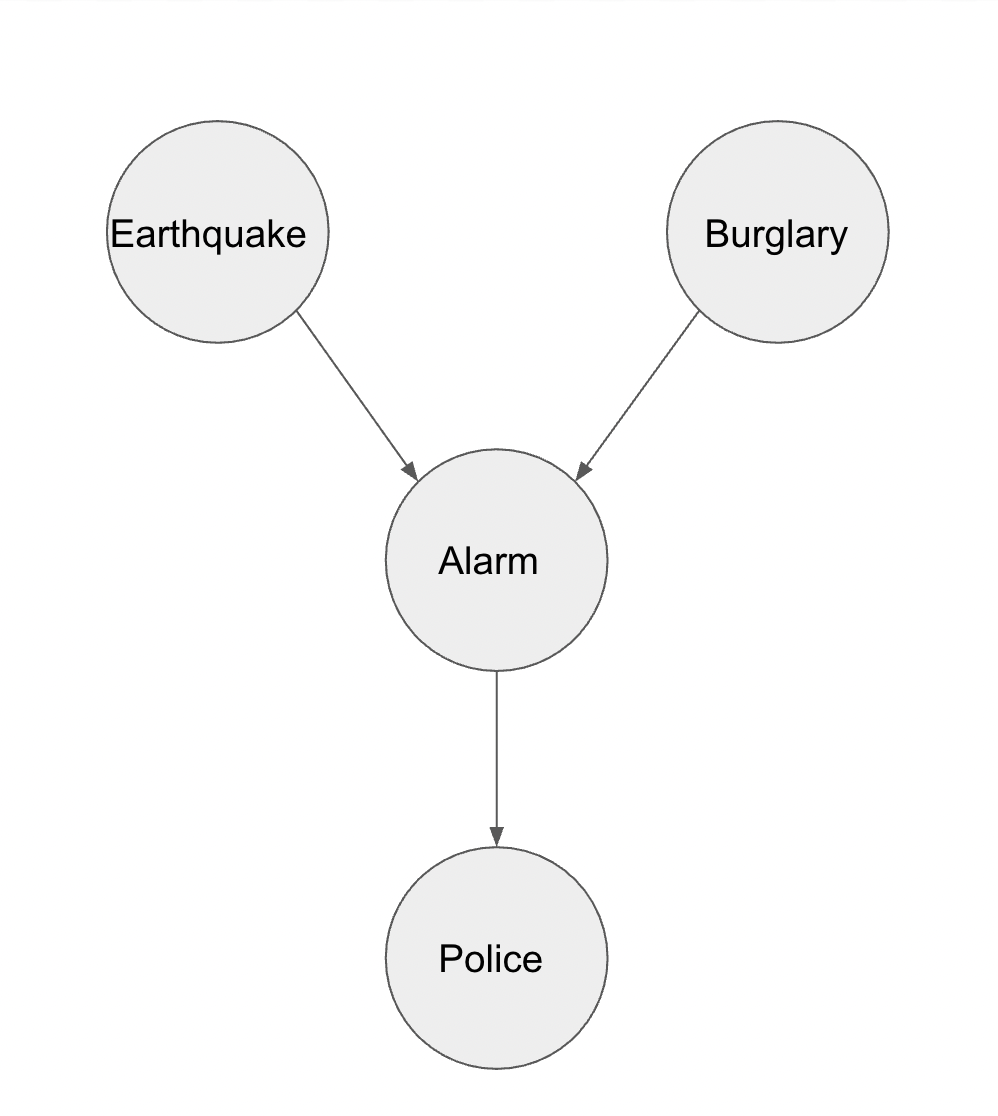
\includegraphics[width=0.3\linewidth]{{figures/BayesNet}}
        \caption{Bayesian network describing the causal relationship between the causal factors.}
        \label{fig:1c}
    \end{figure}

    \begin{figure}
        \centering
        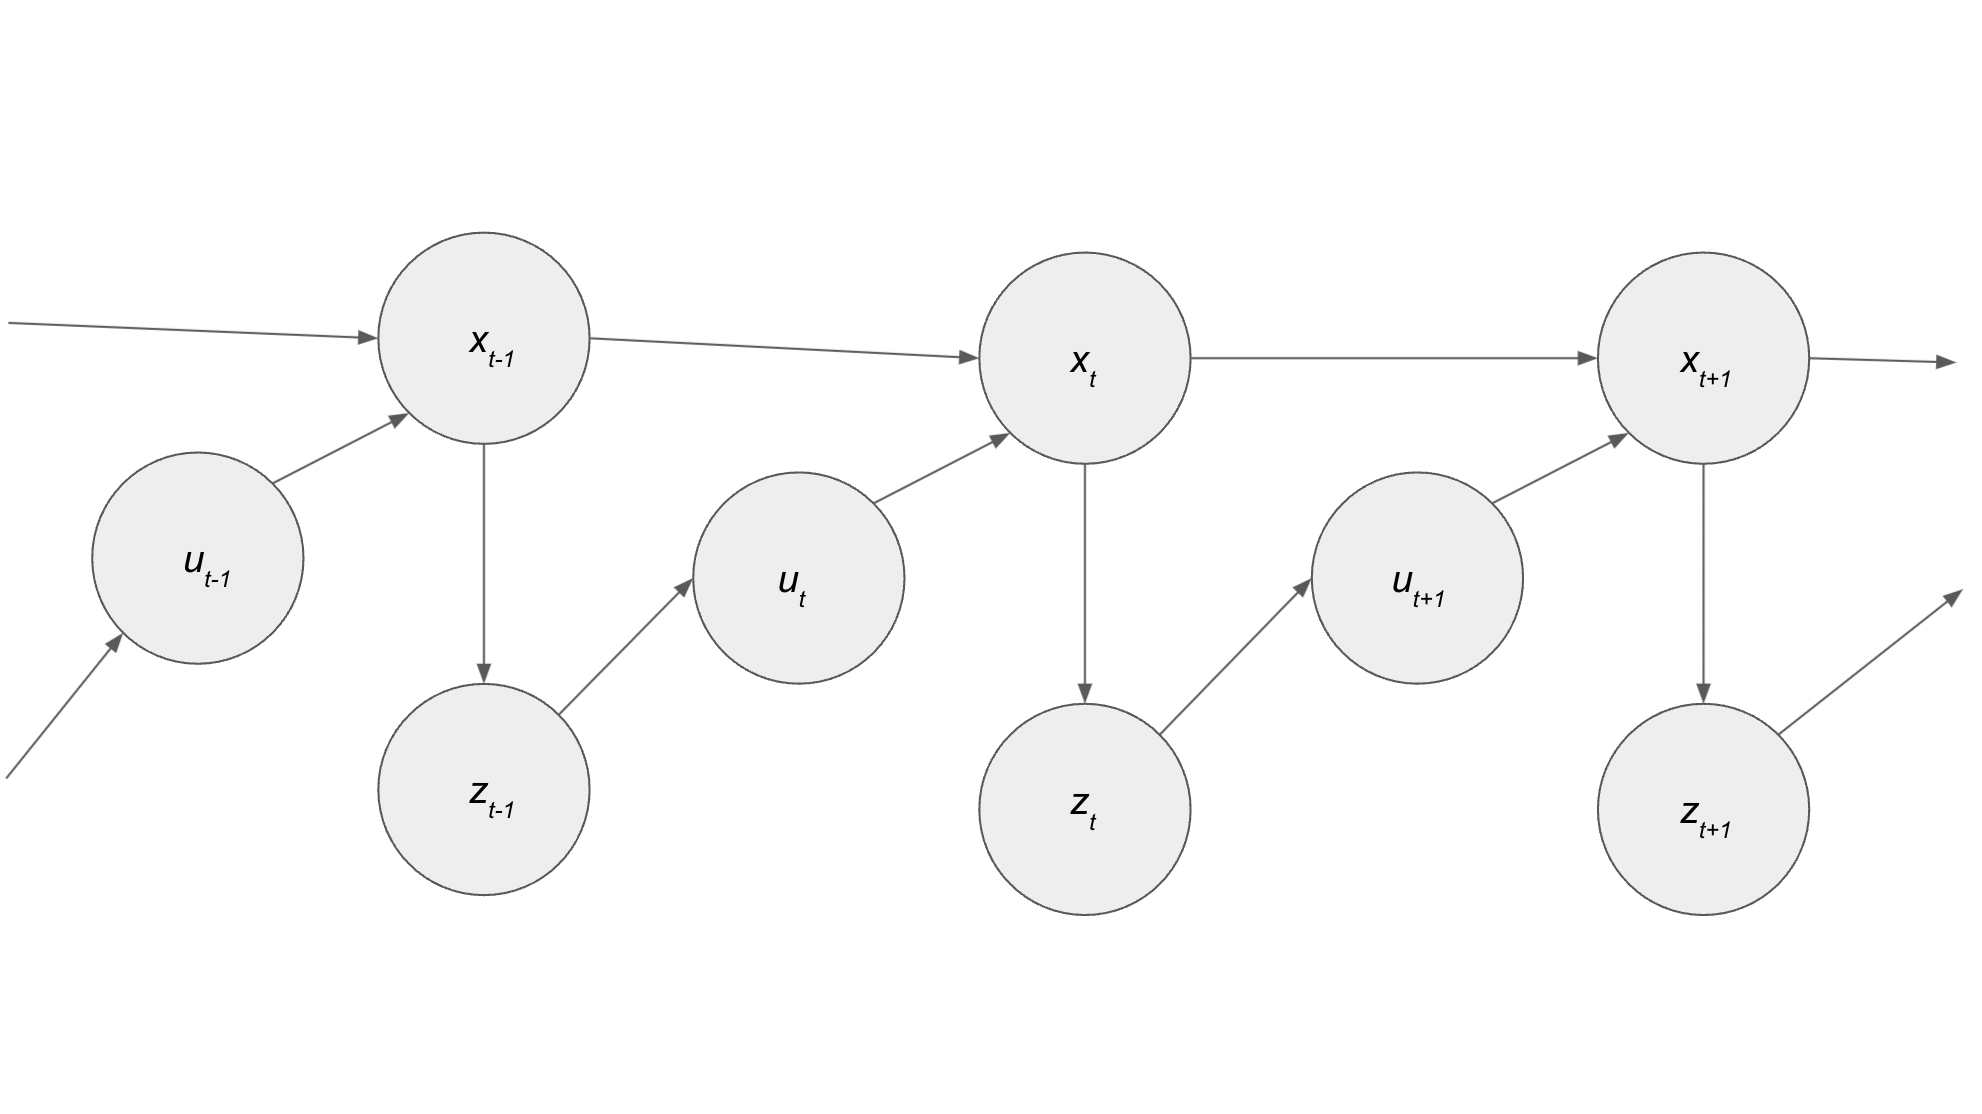
\includegraphics[width=0.8\linewidth]{{figures/BayesNet2}}
        \caption{Bayesian network illustrating recursive state estimation if controls were influenced by observations.}
        \label{fig:1d}
    \end{figure}

    \bigbreak
    \bigbreak

    \begin{question}
        ~%
        \begin{itemize}
            \item[(a)] The vanilla Kalman Filter's (no process noise) position estimate and MSE can be seen in Figure \ref{fig:2a}, and in \texttt{$\sim$/code/} directory of the Github repo.

            \item[(b)] See Figure~\ref{fig:2bb} for MSE plot.
        \end{itemize}

    \end{question}

    \begin{figure}
        \centering
        \begin{subfigure}[b]{0.45\textwidth}
            \centering
            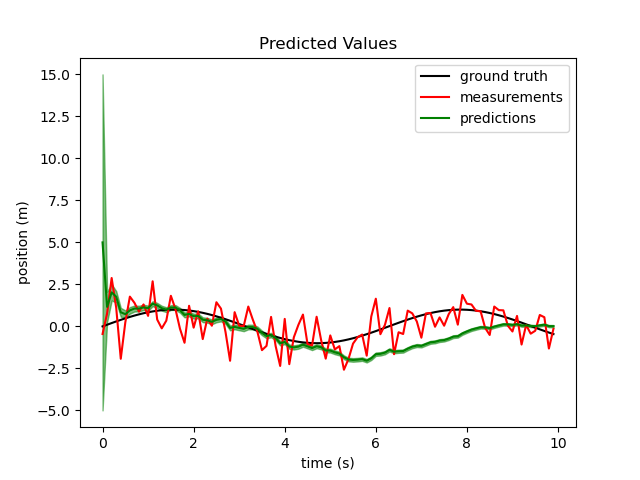
\includegraphics[width=\textwidth]{{code/problem2a_kf_estimation.png}}
            \caption{Evolution of the estimated position and confidence over time.}
        \end{subfigure}
        \begin{subfigure}[b]{0.45\textwidth}
            \centering
            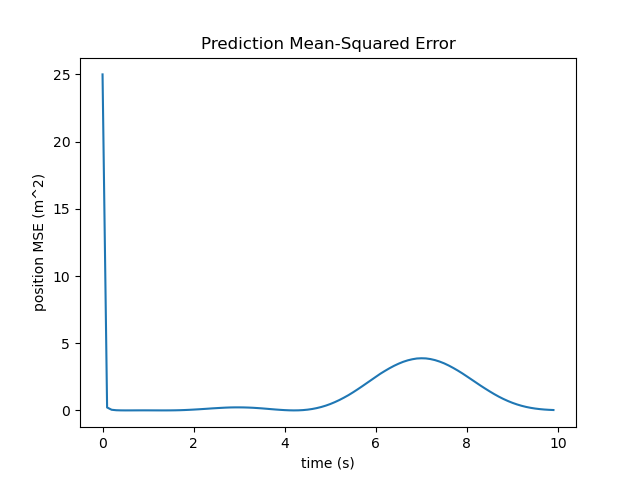
\includegraphics[width=\textwidth]{{code/problem2a_kf_mse.png}}
            \caption{Mean Squared Error of the position of the object, average over $N = 10,000$ trials.}
        \end{subfigure}
        \caption{Figures for Problem 2(a).}
        \label{fig:2a}
    \end{figure}

    \begin{figure}
        \centering
        \begin{subfigure}[b]{0.45\textwidth}
            \centering
            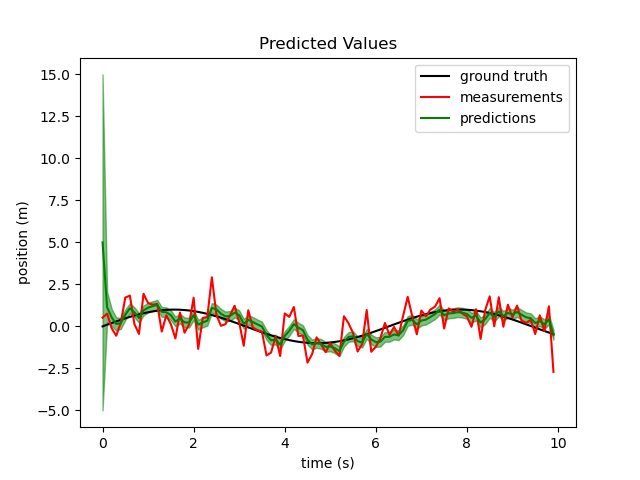
\includegraphics[width=\textwidth]{{code/problem2b_kf_estimation.png}}
            \caption{Evolution of the estimated position and confidence over time.}
        \end{subfigure}
        \begin{subfigure}[b]{0.45\textwidth}
            \centering
            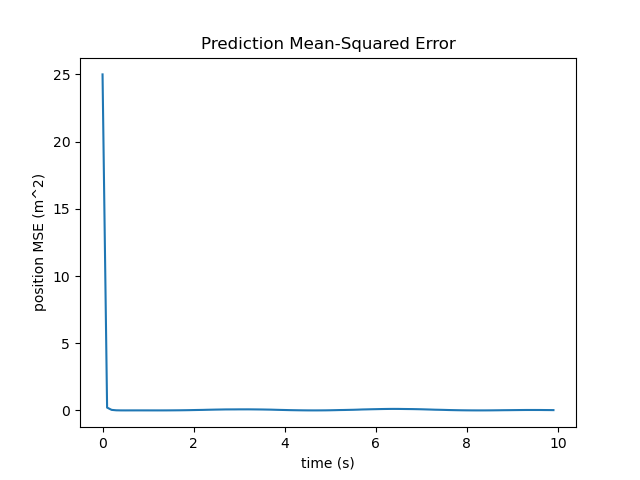
\includegraphics[width=\textwidth]{{code/problem2b_kf_mse.png}}
            \caption{Mean Squared Error of the position of the object, average over $N = 10,000$ trials.}
            \label{fig:2bb}
        \end{subfigure}
        \caption{Figures for Problem 2(b).}
        \label{fig:2b}
    \end{figure}

    \newpage

    \newpage
    \begin{question}
        ~
        \begin{enumerate}
            \item[(a)] We can estimate the parameter $\alpha$ of the scalar system 
            \begin{align*}
                x_{t+1} &= \alpha x_t + \omega(t) \\
                z_t &= (x_t^2 + 1)^{1/2} + \nu(t)
            \end{align*}
            by modeling the system as an Extended Kalman Filter. 
            
            Let $\vb{x}_t = \transpose{\colvec{x_t & \alpha_t}}$ denote the state vector at time $t$. Let $\vb{\mu}_t = \colvec{\mu_t^{(x)} & \alpha_t}^T$ be a random variable from a normal distribution denoting our belief of the state at time $t$. Then our system is characterized by the following nonlinear system.
            \begin{align*}
                \vb{x}_{t+1} &= \vb{g}(\vb{x}_t) + \omega(t) \\
                \vb{z}_t &= \vb{h}(\vb{x}_t) + \nu(t) \\
                \vb{g}(\vb{x}_t) &= \colvec{ \alpha_t x_t  \\ \alpha_t} \\
                \vb{h}(\vb{x}_t) &= \colvec{(x_t^2 + 1)^{1/2} \\ 0}
            \end{align*}
            In order to linearize our system, we can perform a first-order Taylor expansion about the current belief at that timestep, $\mu_t$.
            \begin{align}
                \vb{g}(\vb{x}_t) &\approx \vb{g}(\vb{\mu}_t) + G_t(\vb{x_{t-1} - \mu_{t-1}}) \\
                \vb{h}(\vb{x}_t) &\approx \vb{z}(\bar{\mu}_t) + H_t(\vb{x_{t-1} - \bar{\mu}_{t-1}})
            \end{align}
            where $G_t, H_t$ are the gradients of $\vb{g}, \vb{h}$ evaluated at the current belief $\mu_t$, respectively.
            \begin{align}
                G_t &= \colvec{\alpha_t & \mu_t \\ 0 & 1} \\
                H_t & = \colvec{\frac{\bar{\mu}_t}{\sqrt{\bar{\mu}_t^2 + 1}} & 0 \\ 0 & 0}
            \end{align}
            Note that $\vb{h}$ and its gradient are evaluated at $\bar{\mu}_t$, which is the current belief of the model at the time of linearizing the function.

            Now we can use $\vb{g}, \vb{h}, G, H$ in the EKF algorithm to estimate the parameter $\alpha$, which would be the second element in the predicted state vector.

            \item[(b)] Since the ground truth itself is stochastic, the performance of the EKF varies drastically from one run to another. One issue that arises is, as the predicted position approaches zero, the model can no longer update its estimate of $\alpha$. Since position is used to estimate the parameter $\alpha$ (in $\vb{g}$), the filter can no longer update its estimate after a few timesteps when the predicted position goes to zero. See Figure~\ref{fig:3b} for estimate plot.
        \end{enumerate}
    \end{question}

    \begin{figure}
        \centering
        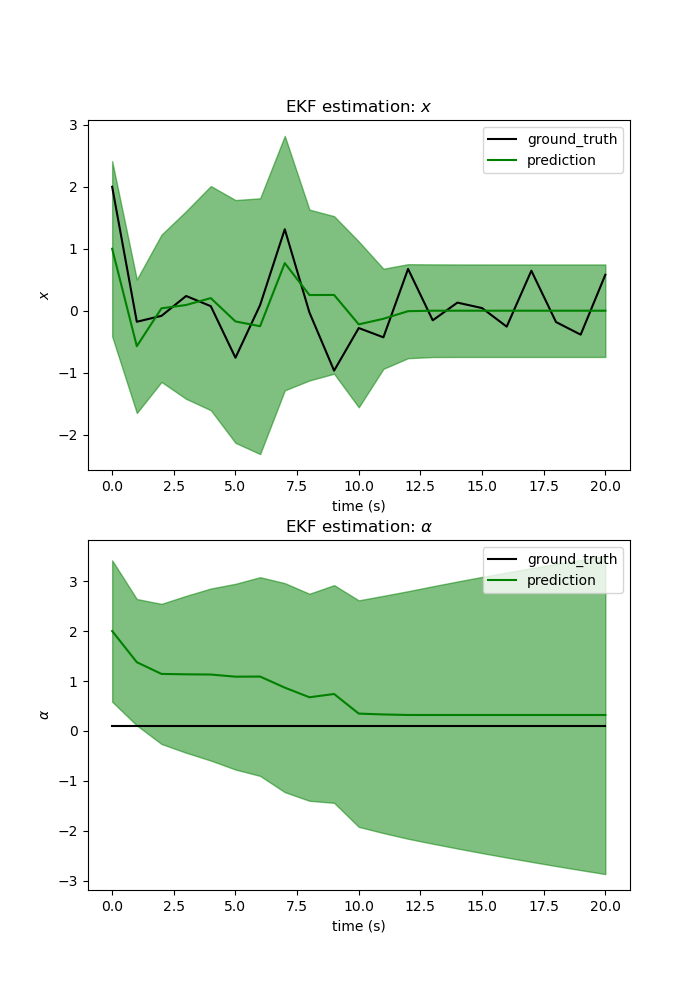
\includegraphics[width=0.8\linewidth]{{code/problem3_ekf_estimation}}
        \caption{Extented Kalman Filter estimate of position $x_t$ and parameter $\alpha$.}
        \label{fig:3b}
    \end{figure}



\end{document}
